\setcounter{chapter}{6}


\chapter{Discussion and Future Work}
\label{ch:discussion}

In conducting the studies reported on in
this dissertation and in developing the
techniques explored, we made many decisions.
In this chapter, we discuss the limitations
and trade-offs that resulted and discuss
future avenues for exploration.

%In this chapter, we discuss questions
%and decisions not addressed in the previous chapters of this dissertation. 
%We also use this discussion to describe potential venues for future work.

% characterization of task-relevant text across multiple artifact types,
% in the design of the semantic-based techniques that we have explored, 
% or in our empirical evaluation of \acs{tool}.



 


% potential improvements to the semantic-based
% techniques. We also introduce potential tools
% that can leverage the broader applicability
% of the semantic-based techniques.







%\section{Limitations \& Trade-offs}
\section{Relevance}
\label{cp7:relevance}

A primary assumption in this dissertation
is that there will be text in documents
associated with a software development
task that is commonly seen as \textit{relevant}
to the task. Chapter~\ref{ch:characterizing} demonstrates
that sufficient commonality of relevant
text does exist to support the development
of techniques and Chapter~\ref{ch:assisting} shows
that the automatically identified text
is seen as relevant. For instance,
some participants in the \acs{tool}
experiment indicated:

\smallskip
\begin{quote}
    ``\textit{The highlights were super useful, without them I would definitely had not been able to rapidly do the task.}''---P9
\end{quote}


\begin{quote}
``\textit{With the highlighted references, I was able to move much quicker. I quickly glanced at each resource, reading just the highlights to determine how valuable that resource was. The highlights allowed me to focus on the most relevant resources, gathering the necessary information to complete the task. 
}''---P15
\end{quote}

Yet, others who participated in the \acs{tool}
experiment disagreed with the concept that text
in these documents was important at all:





\smallskip
\begin{quote}
``\textit{I realized going through [the experiment] that I read very little free-form text when looking for solutions. Mainly code samples with clear, succinct examples or type/method definitions.}''---P12
\end{quote}

\begin{quote}
``\textit{I'm not going to bother reading the text if I don't have to, especially when the code snippets are easy to understand.}''---P16
\end{quote}




\smallskip
This feedback suggests that the kind of information considered useful in a document not only differs based on 
a developer's  \textit{explicit} versus \textit{implicit} reasoning, but also that it varies with the developer. 
It suggests that techniques will need to
be even more general to work across document
types: techniques will also need to work across
the different kinds of information in a document.
Future studies should more deeply investigate
the kinds of information developers deem as
relevant and explore how developers gauge relevance.





How and what developers consider relevant in
documents may also impact how techniques trade-off
precision versus recall. 
In Chapter~\ref{ch:identifying}, we indicated
the techniques we explored favored locating
all relevant text within an
artifact, in other words recall, rather
than focusing on 
correctly determining relevant text, in other
words precision. 
We made this decision because, as described in 
 (Chapter~\ref{ch:introduction}),
missing relevant text would mean that a developer might have an incomplete or partial view of the information needed, which may lead to
sub-optimal decisions.




% (i.e., a developer might have to perform further searches and perhaps revisit artifacts that they have already inspected)

However, when favoring recall,  we may obtain more false positives; non\-/relevant text indicated as relevant.
Due to the limited time developers spend inspecting a natural language artifact~\cite{Starke2009}, there is a chance that
 a developer could discard reading an artifact due to a false positive. 
 Although abandoning reading an artifact and moving to another artifact could lead to non\-/efficient work,
we believe that the benefits of automatically identifying relevant text outweigh these risks. 
Inspecting an artifact without tool support is more time\-/consuming
than inspecting each sentence retrieved to judge their relevance to the task at hand. 
Future studies could explore the ramifications
of this trade\-/off in detail.







%This feedback suggests that we could have observed different usage behaviours if participants had the chance to decide when to invoke \acs{tool}.
%However, 
%our experimental design focused on comparing tasks using or not \acs{tool} and thus, participants did not have the option to 
%request \acs{tool} to automatically identify task-relevant text on the fly. 


%To understand who would use  \acs{tool} in which types of tasks or 
%what factors  influence the tool's usage,
%we would have to consider a different experiment with challenges and risks of its own.
%For example, designing a longitutional study investigating how developers 
%with different expertise and background
%of some open source community would use \acs{tool}.



% This feedback also brings to light one core limitation of our techniques:
% automatically identifying text relevant to a task is of little to no help
% to developers who focus on code snippets or to developers who disregard 
% reading the text in a natural language artifact.




%\paragraph{\textbf{Precision vs Recall.}}
\section{Technique Deployment}
\label{cp7:deployment}

%\paragraph{\textbf{Training Data.}}

% \gcm{I think both training data and costs are
% more about how you would actually deploy
% your technique. I'm a bit confused
% on the training data whether you are suggesting
% that the technique needs to be trained on
% project-specific data?} \art{not project specific data, 
% but it need training samples as the ones in the 
% datasets that we produced}


% make it more explicit, dev ops example is a good idea

% \gcm{On Costs, I'm a bit
% confused as to whether needing a server 
% is just because of current hardware that
% might be eased in the future.} \art{for now, yes}

In Chapter~\ref{ch:identifying}, we have shown that semantic-based approaches identify task-relevant textual information across
different types of artifacts without relying on
assumptions about the nature of an artifact or its meta-data.
However, we
observe that the techniques with the best accuracy require fine-tuning 
a deep learning model
and this could be considered as an impediment to deploying such techniques. 


Fine-tuning requires training data---tasks, natural language artifacts, and text annotated as relevant---and
one potential limitation arises from how the training data might lead the model to identify 
text that is not relevant to certain types of tasks.
For example, with the adoption of Agile practices~\cite{fowler2001agile} and continuous  delivery~\cite{humble2010continuous}, 
there has been a rise in automated approaches for organizing and facilitating 
continuous delivery, which are commonly referred to as \textit{DevOps}~\cite{senapathi2018devops, leite2019ops}.
DevOps tasks and natural language artifacts documenting DevOps tools 
might significantly differ from tasks and artifacts associated with bug fixing or implementing new features
and, despite the fact that we observed that a model fine-tuned with 50 Android tasks 
was able to identify text relevant to Python tasks (Figure~\ref{fig:eval-comparison}), 
it is not clear if a model fine-tuned with certain data is able to identify text relevant to tasks 
in a different context. 
Future research should more deeply investigate the extent to which 
tasks and artifacts affect the task-relevant text identified by a model 
that requires fine-tuning.







A second limitation to deploying the techniques we explored
relates to the current cost associated with deep learning models. 
The neural embeddings and the neural networks we used
 often requires dedicated servers with significant 
memory and high-throughput computational power.
 Due to the high demand for commercial servers with such properties, 
 it might be difficult to deploy our tools for usage a large scale.
We believe that hardware cost might be eased in the future.
% \art{I simplified the cost paragraph, but it might still be better to remove it}



% The need for dedicated servers also means that our proposed techniques and our web browser plug-in cannot run offline. If we consider a standard client-server architecture, such as the one of \acs{tool}, it means that one must send data about the task and artifacts that they are working to a remote server for processing. This might not always be possible due to privacy reasons, i.e., outside the public domain, organizations would not be willing to use our tool and, depending on their size,  organizations might not have the resources needed for in-house solutions. Due to these limitations, the techniques and tools described in this dissertation 
% must be treated as proofs-of-concept and we hope that 
% these limitations might be eased in the future.


\section{Future Work}
\label{cp7:future-work}



In this section, we elaborate some of the future research  
mentioned in Sections~\ref{cp7:relevance} and~\ref{cp7:deployment}.
We also discuss other avenues for future work.


\subsection{Relevance Datasets}
\label{cp7:gauging}


In Section~\ref{cp7:relevance}, we indicated that future studies should further investigate 
what kind of information developers deem relevant and how developers gauge relevance.
Upon reflecting on the data-gathering procedures described throughout this work,
a potential line of work is to consider 
gathering data from software professionals performing daily tasks in a non-obstructive way.



Conducting empirical
 experiments in a more realistic environment is challenging~\cite{Kevic2015}.
This effort is worthwhile as
the richness of collected data can provide valuable insights
to provide a foundation for tool development.
One potential method for
data collection 
considers 
how recent studies with eye-trackers~\cite{Cutrell2007, Petrusel2013, sharafi2020}
have shown that the technology is not as disruptive as other 
methods~\cite{Lazar2017} such as think aloud protocols or manual input. 
Hence, we believe that eye-tracking 
could be used in a developer's working environment, 
leading to more realistic data on which text developers perceive as task-relevant.
For example, one could
extend the work done by Kevic and colleagues on
tracing developers' eye for change tasks~\cite{Kevic2015} to
also consider tracing data outside a developer's IDE
for such a purpose.



A second venue is to consider who perceived which text as relevant.
As observed both in related work~\cite{Crosby1990, Busjahn2015} and in our formative study (Chapter~\ref{ch:characterizing}),
there is variability in what text may be relevant to a software task and 
providing more background data about 
the participants who considered some information useful could lead to benchmarks 
for evaluating techniques
focused on a certain population (e.g., expert versus novice developers~\cite{Crosby1990, Busjahn2015}). 



% In Chapter~\ref{ch:related-work}, we described 
% a series of studies that mine text from natural language artifacts.
% These studies provide annotated data 
% resulting from coding procedures that usually do not take into account
% differences in what might be relevant; or disagreements are resolved during the annotation process. 
% However, in our formative study (Chapter~\ref{ch:characterizing}),
% we have observed that there is variability in what text may be relevant 
% to a software task, a fact that other researchers have also brought to light~\cite{Bavota2016,Robillard2015}.









\subsection{Sentence Semantics}
\label{cp7:semantics}




In Chapter~\ref{ch:characterizing}, we used frame semantics, a general linguistic approach~\cite{fillmore1976frame},
as a means for access to the meaning of the text in natural language software artifacts.
However, questions remain about whether
semantic frames can help in identifying the semantics of software engineering text
and the extent to which it applies to software engineering text.




We partially addressed these questions in a study, 
orthogonal to this dissertation~\cite{marques2021},
where we assess the applicability of generic semantic frame
parsing to software engineering text
aimed at supporting program
comprehension activities.
In this study, we first assessed how the tool we used in Chapter~\ref{ch:characterizing}
to analyze the meaning of the text considered relevant (i.e., SEMAFOR~\cite{das2014frame})
 applies to text sampled from 1,802 documents drawn from a set of datasets~\cite{Arya2019, Xu2017, Maalej2013, Chaparro2017}. 
Based on the results from this analysis, 
we proposed \textit{SEFrame}, a tool that tailors 
frame parsing to natural language text in software engineering artifacts.
Results from a second evaluation indicated that \textit{SEFrame} was 
 correct in between 73\% and 74\% of
the cases and that it parsed text from a variety of software artifacts used to support program
comprehension, which motivated our decision to apply \textit{SEFrame} 
in the design of the techniques we explored in Chapter~\ref{ch:identifying}.
Future research should consider
a more in depth investigation of 
frame semantics or other general approaches that can infer the meaning of text at the sentence level. 


For example, future studies could focus on answering 
which frames most accurately capture the information conveyed in the text 
and how frames extracted by state-of-the-art tools (e.g.,~\cite{swayamdipta17, chen2021joint})
compare to manual labels provided by researchers 
about the information available in certain kinds of software artifacts~\cite{Maalej2013, Arya2019, Sorbo2015}.  



 






\subsection{Deep Learning for Software Engineering}
\label{cp7:deep-learning}



Future research in the field of deep learning for software engineering could consider 
exploring other pre-trained \acs{DL} models as well as other applications of 
deep-learning to software engineering tasks. 




In Chapter~\ref{ch:identifying}, we have discussed threats associated with the BERT pre-trained model 
we used and how future research should consider other 
general or software-specific pre-trained models.
We did not explore other general pre-trained models because most of the models that apply to our domain problem 
are variations of BERT (e.g., Albert~\cite{lan2019albert} or Roberta~\cite{liu2019roberta})
and by using the BERT base model, we sought to establish a baseline for future comparisons.




With regards to software-specific models (e.g., ~\cite{feng2020-codebert, li2019neural}), we also emphasize 
that these models have been trained on either source code or source code and method level text documentation. 
These datasets might not align with how developers discuss text in natural language artifacts~\cite{arya2020}, such 
as Stack Overflow posts or web tutorials. Therefore, future research should consider how 
 models pre-trained on text originating from various kinds of 
natural language software artifacts compare to the base model that we used.





In Chapter~\ref{ch:identifying}, we have shown that artifact-specific techniques, such as AnswerBot, have accuracy comparable to the semantic-based approaches
we have explored. This  provides
a unique opportunity for the creation of synthetic data that we can use to further fine-tune the deep-learning models we explored.
For that, future research should show that models trained on synthetic data
 extend beyond what an artifact-specific technique used for bootstrapping already provides. For example, showing that
a model fine-tuned using synthetic data can identify task-relevant textual information in a different type of artifact or showing
that the model's accuracy is significantly better than the technique used for bootstrapping.


% \art{Think whether I need anything else in this section}


% As  other potential applications of \acs{DL}, we highlight how researchers can use BERT's attention mechanism~\cite{Vaswani2017attention}
% in software engineering activities such as finding who should fix a bug~\cite{anvik2006}, requirements traceability~\cite{Lin2021}


% in sentence pairs. As we have described in Section~\ref{cp5:approach-bert}, we used this mechanism to correlate the text in natural language artifacts and the text in a task and future research could explore applying attention for recommending  
% or in other words pairing the text in 
% or 








\subsection{Presenting Task-Relevant Text}
\label{cp7:info-viz}




In Chapter~\ref{ch:assisting}, we described how \acs{tool}
highlights the text in a natural language artifact that it identifies 
as relevant to an input task. Our idea to highlight text 
draws from related work which suggests that textual highlights 
are a simple approach to surface the most important information in 
an artifact~\cite{Robillard2015,nadi2020}. 
Although simple, participants shared limitations of 
this strategy:



\smallskip
\begin{quote}
``\textit{It was much easier to follow with previously highlighted text.  
    However, it would have been nicer to have some sort of side bar/index of highlighted snippets
    where I could know and scroll directly through the highlighted parts of a page.}''---P9
\end{quote}



\smallskip
\begin{quote}
``\textit{There was a resource page which was super long, and I found it very difficult to locate which sentences were highlighted, therefore, making that resource useless to me because I didn't have the motivation to scroll through it to find all highlights. An interface that gathers highlight locations would make a difference.}''---P21
\end{quote}


\smallskip
This feedback made us question other potential ways to present the text identified by \acs{tool}.
For example, we could have followed design principles adopted by Unakite~\cite{Liu2018Unakite}---a tool that collects, organizes and keeps track of information---to make \acs{tool} display the text identified on its context menu.
Figure~\ref{fig:navigational-cues} shows a mock up of \acs{tool} bundling the highlights identified for one of the artifacts in the \texttt{titanic} task (Section~\ref{cp6:tasks}).
Using this context menu, a user could click on the text identified and navigate to the part of the documentation 
originally containing the text.



\begin{figure}[H]
    \centering
    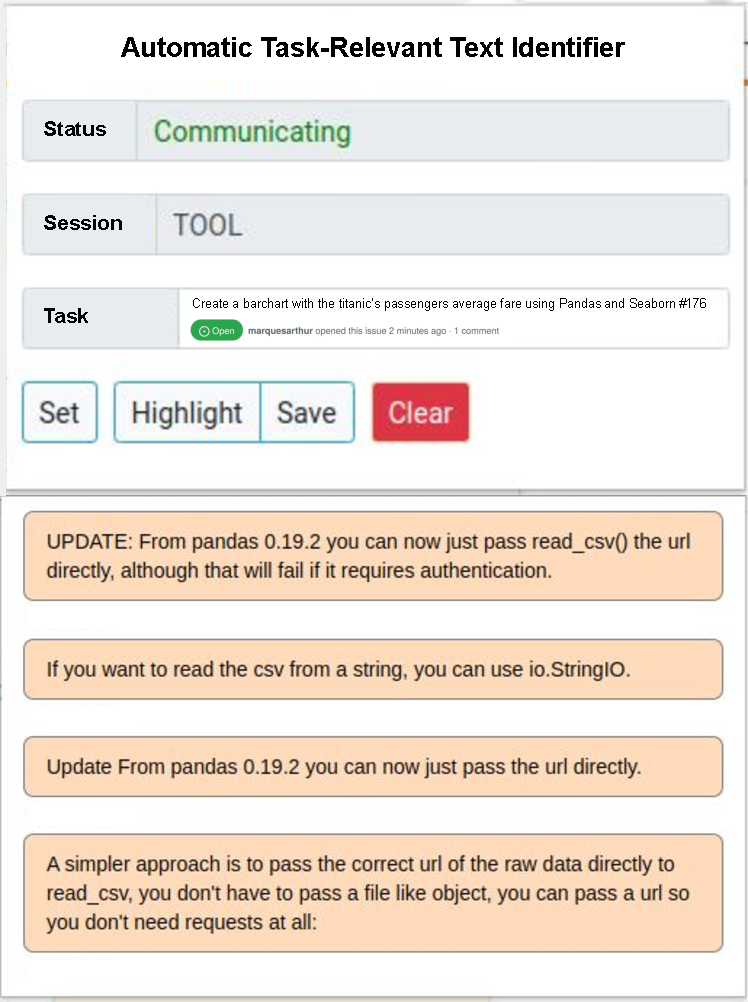
\includegraphics[width=0.55\textwidth]{fig/cp7/navigational-cues}
    \caption{Mock up of the highlights identified by \acs{tool} as navigational cues; by clicking on a highlight, a user could be directed to the part of a document containing that highlight}
    \label{fig:navigational-cues}
\end{figure}



A second approach to organizing the text identified could consider 
the semantic meaning of each sentence, as extracted through frame semantics or other semantic-based approaches. 
Semantic frames could 
assist a user in comprehending the content of the text automatically identified
without the need to read it. 
As done by Libra~\cite{Ponzanelli2017}, semantic frames could also be used to group the text identified in bubbles or a hierarchical representation 
 helping a developer
in deciding what portions of the text they would inspect first. 
Figure~\ref{fig:semantic-cues} shows a mock up 
with some of the semantic frames extracted 
for the sentences in Figure~\ref{fig:navigational-cues}.
Using the semantic frames identified,
a developer could decide whether they would read sentences 
describing some coding procedure (\textit{execution}), or sentences 
with warnings or requirements about the Pandas API (\textit{requirement} and \textit{being obligated}). 
To be useful, future research must consider how to identify from all the frames available in a sentence, 
which frames
better summarize the meaning of the text. 


We leave the investigation of other ways to present task-relevant text to future research.




\begin{figure}
    \centering
    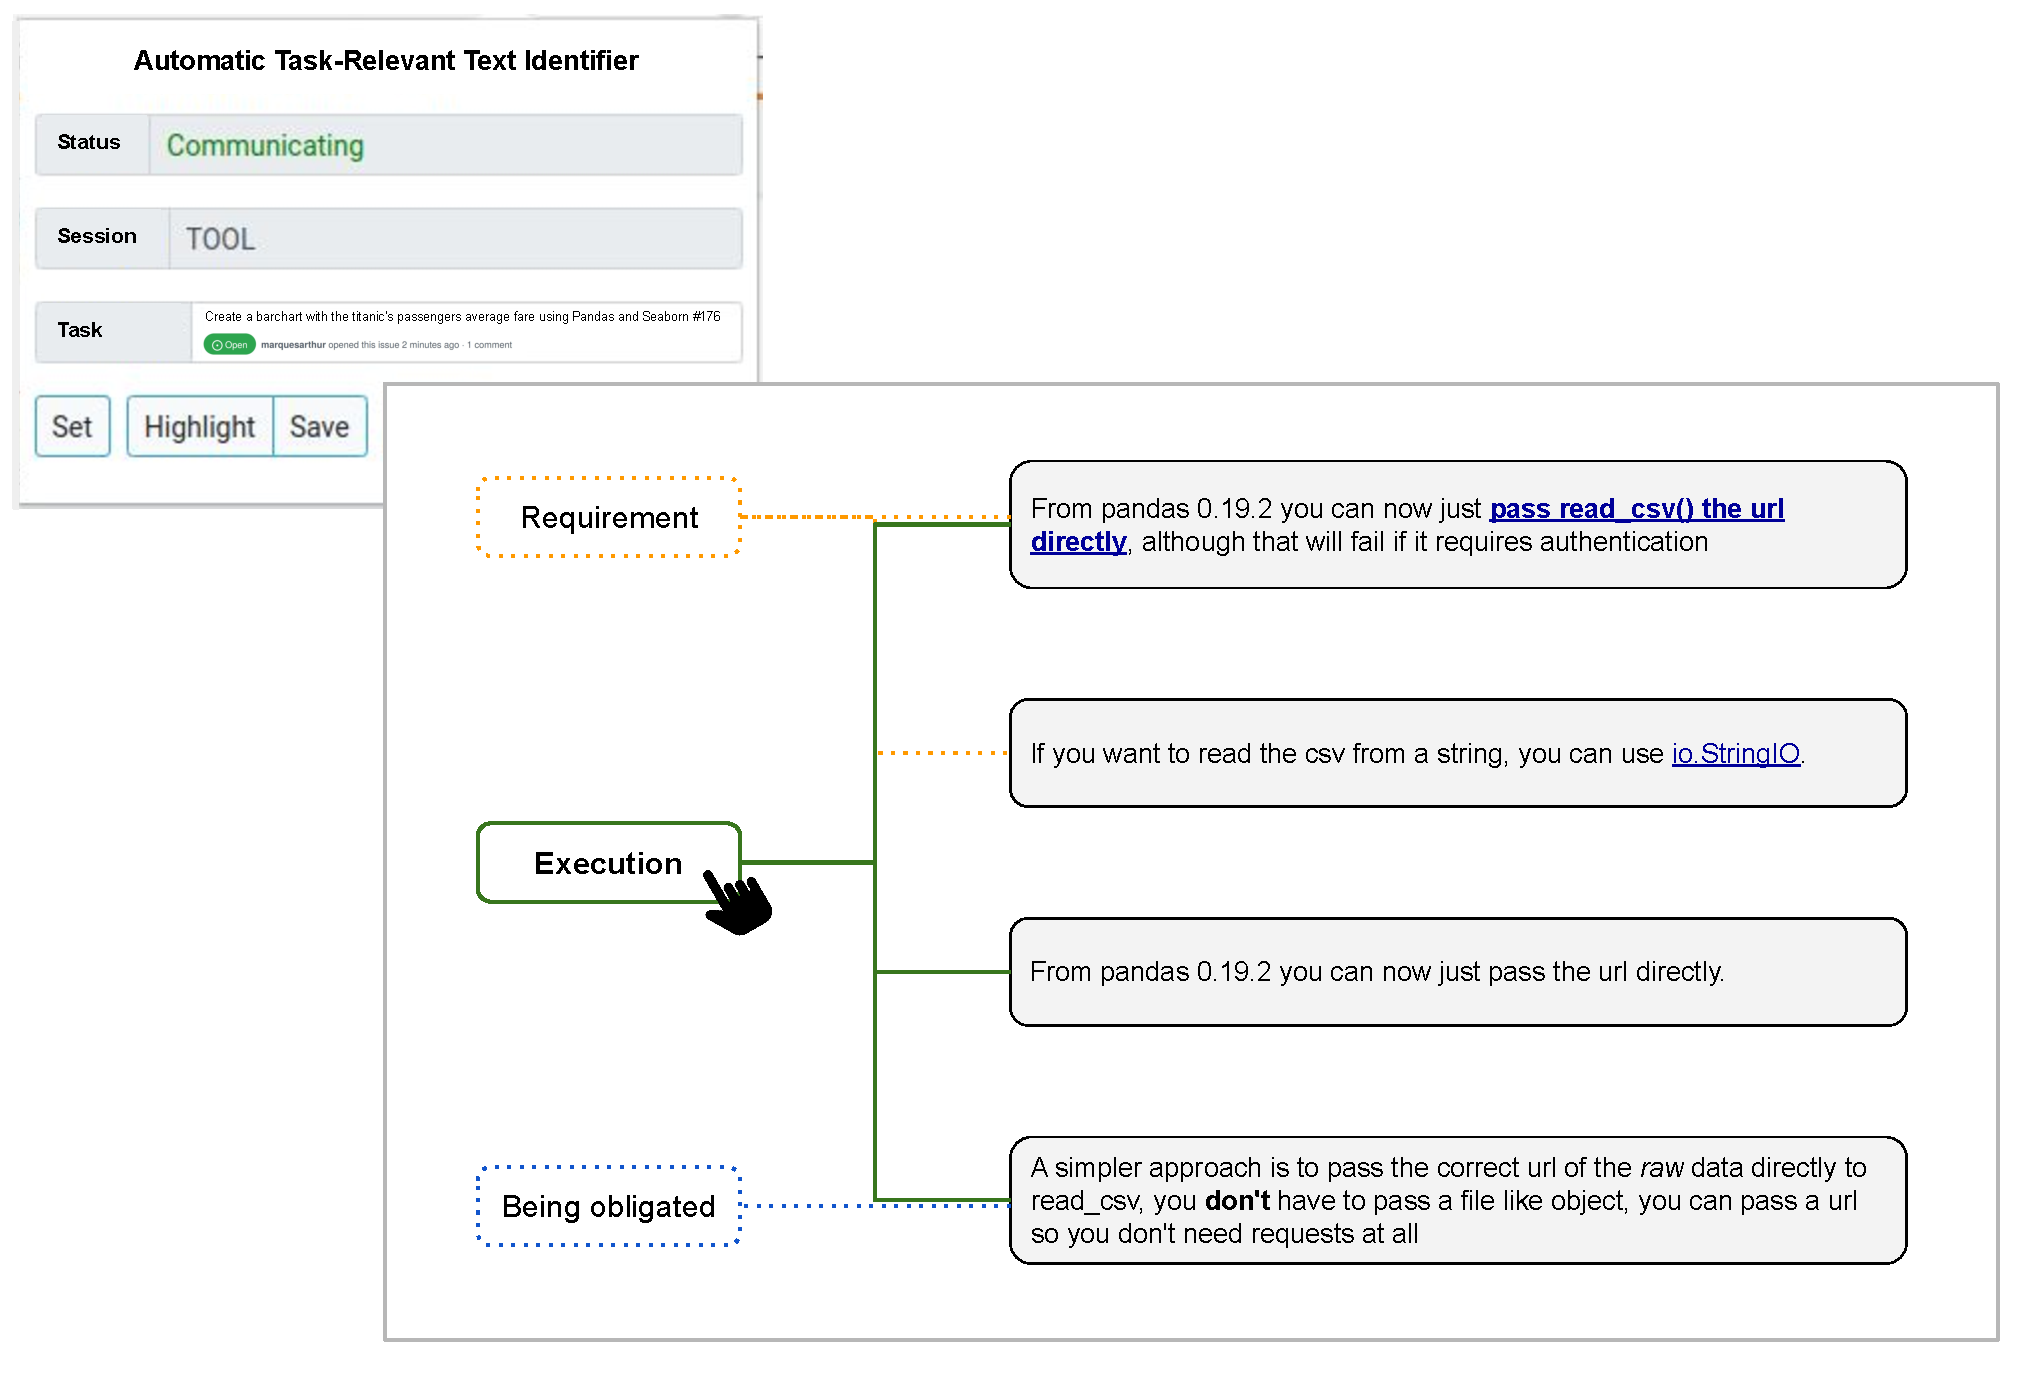
\includegraphics[width=0.90\textwidth]{fig/cp7/semantic-cues}
    \caption{Mock up of the highlights grouped by semantic frames; by hovering over a semantic frame, a user could quickly identify which of the text identified is associated with a certain meaning}
    \label{fig:semantic-cues}
\end{figure}








% 

\section{Semantics in Software Development Artifacts}
\label{cp7:semantics}



In Chapter~\ref{ch:characterizing}, we used frame semantics---a general
linguistic approach---to infer the meaning of the sentences
that developers deemed relevant to complete a software task.
As one potential alternative to this approach, 
we could have considered the taxonomies available 
in other studies such as the knowledge types in API documents~\cite{Maalej2013}
or the information types in Open Source GitHub issues~\cite{Arya2019} or 
in development mailing lists~\cite{Sorbo2015}.


We decided to not use such taxonomies because the categories available in these and other studies 
are often based
on a need for access to the meaning of
sentences in the natural language text
and we were interested in assessing the
applicability of generic semantic frame
parsing for this purpose.
To the best of our knowledge, there have been only a few uses of frame
semantics in software engineering research~\cite{jha2017, kundi2017, alhoshan2019using}
and these approaches
have largely focused on text associated
with software requirements, leaving open the
question of applicability of the approach to
text in different kinds of natural language artifacts.





Motivated by our findings on the semantic analysis of the relevant text 
found in API documents, GitHub issues, and \acs{qa} pages, 
we addressed the question of whether semantic
frames can help identify the meaning of
software engineering text
in a study 
orthogonal to this dissertation~\cite{marques2021}. 
In this study, we assessed the applicability of generic semantic frame
parsing to software engineering text
aimed at supporting program
comprehension activities.
First, we assessed how the tool we used in our semantic analysis, i.e., SEMAFOR~\cite{das2014frame},
 applies to text sampled from 1,802 documents drawn from existing datasets~\cite{Arya2019, Xu2017, Maalej2013, Chaparro2017}. 
Based on the results from this analysis, 
we proposed \textit{SEFrame}, a tool that tailors 
frame parsing to natural language text in software engineering artifacts.
We assessed the correctness and robustness of \textit{SEFrame} in a second evaluation where we found that the approach was 
 correct in between 73\% and 74\% of
the cases and that it can parse text from a variety of software artifacts used to support program
comprehension. These results motivated our decision to apply \textit{SEFrame} 
in the design of the techniques we explored in Chapter~\ref{ch:identifying}.
Nonetheless,  
future research could consider more complex and modern 
frame semantic parsing tools (e.g.,~\cite{swayamdipta17, chen2021joint}) to more
accurately classify the semantic information in software engineering
text and other potential applications 
of frame semantics to software engineering problems.
 





% 


\section{Deep Learning Models for Software Engineering Tasks}
\label{cp7:deep-learning}
% 






\section{Empirical Studies on Determining Relevancy}
\label{cp7:empirical-studies}


% By reflecting 
% on what is relevant, 
% the annotated data in ou corpora is an approximation 
% of what developers implicitly find relevant to a task. 



At multiple points in this dissertation, participants produced annotated data 
indicating the text that they deemed relevant to a software task. 
These annotations reflect their \textit{explicit} reasoning about the information 
available in the text and what they consider relevant to the tasks 
that we presented them. 
Due to differences that might arise from explict and implicit reasoning,
 we argue for the need for more empirical data 
originating from
software developers performing daily tasks
and gathered in a non-obstructive way.
Conducting empirical
 experiments in a more realistic environment is challenging~\cite{Kevic2015}.
This effort is worthwhile as
the richness of collected data can provide valuable insights
to provide a foundation for tool development
and eye-tracking~\cite{Cutrell2007, Petrusel2013, sharafi2020}
is a promising approach to collect more realistic data without disrupting a developer's workflow.
For example, one could
extend the work done by Kevic and colleagues on
tracing developers' eye for change tasks to
also consider tracing data outside a developer's IDE~\cite{Kevic2015}
for such a purpose.


In Chapter~\ref{ch:related-work}, we described 
a series of studies that mine text from natural language artifacts.
These studies provide annotated data 
resulting from coding procedures that usually do not take into account
differences in what might be relevant. 
In contrast, in our formative study (Chapter~\ref{ch:characterizing}),
we have observed that there is variability in what text may be relevant 
to a software task and, if future empirical studies
provide more data about who perceived which text as relevant, it could lead to benchmarks 
for evaluating techniques
focused on certain population  (e.g., experts versus novices developers~\cite{Crosby1990, Busjahn2015}). 







% In Chapter~\ref{ch:characterizing}, we have also shown that despite consistency in the key information 
% needed to complete a task, there is variability in what text developers deem relevant to a 
% certain task



% Hence, differences in the annotated data and the information needs 
% or certain population (e.g., experts versus novices developers~\cite{Crosby1990, Busjahn2015})
% might not be captured in the data available in the existing corpora.
% The corpora provided as part of this dissertation 
% differs from such studies by indicating the number of developers that deemed some text relevant.



We leave the investigation of other methods on how to determine which text 
developers deem relevant 
and the creation of benchmarks with different properties
as part of future research.





% In fact, early stages in the design of the 
% \acs{DS-android} corpus (Chapter~\ref{ch:android-corpus}) had considered using 
% an eye-tracker for this purpose.
% However, we were unable to pursue this line of work 
% due to the COVID-19 pandemic and challenges related to
% recruiting participants and conducting an in-person experiments.



% A second challenge on 


% Earlier studies
% on extracting relevant
% text from natural language artifacts have typically
% relied on annotated corpora created using coding guidelines.
% These guidelines have procedures to resolve disagreements and the 
% final corpora often does not include iterations of the data considered relevant 
% throughout the coding process.



% Such observation corroborates 
% findings from other studies which observe that 
% individuals assessing the same artifact may have different
% information needs~\cite{Bavota2016, Walters2014}
% and that there are behaviour differences on how





% 


\section{Identifying All Relevant Text}
\label{cp7:relevant-text}
% 


\section{Specificity or Generality?}
\label{cp7:general-vs-specific}
% 




\section{Presenting Task-Relevant Text}
\label{cp7:info-viz}




In Chapter~\ref{ch:assisting}, we described how \acs{tool}
highlights the text in a natural language artifact that it identifies 
as relevant to an input task. Our idea to highlight text 
draws from related work which suggests that textual highlights 
are a simple approach to surface the most important information in 
an artifact~\cite{Robillard2015,nadi2020}. 
Although simple, participants shared limitations of 
this strategy:



\smallskip
\begin{footnotesize}
\begin{quote}
``\textit{It was much easier to follow with previously highlighted text.  
    However, it would have been nicer to have some sort of side bar/index of highlighted snippets
    where I could know and scroll directly through the highlighted parts of a page.}''
\end{quote}
\end{footnotesize}



\smallskip
\begin{footnotesize}
\begin{quote}
``\textit{There was a resource page which was super long, and I found it very difficult to locate which sentences were highlighted, therefore, making that resource useless to me because I didn't have the motivation to scroll through it to find all highlights. An interface that gathers highlight locations would make a difference.}''
\end{quote}
\end{footnotesize}


\smallskip
This feedback made us question other potential ways to present the text identified by \acs{tool}.
For example, we could have followed design principles adopted by Unakite~\cite{Liu2018Unakite}---a tool that collects, organizes and keeps track of information---to make \acs{tool} display the text identified on its context menu.
Figure~\ref{fig:navigational-cues} shows a mock up of \acs{tool} bundling the highlights identified for one of the artifacts in the \texttt{titanic} task (Section~\ref{cp6:tasks}).
A user could click on the text identified and navigate to the part of the documentation 
originally containing the text identified.



\begin{figure}
    \centering
    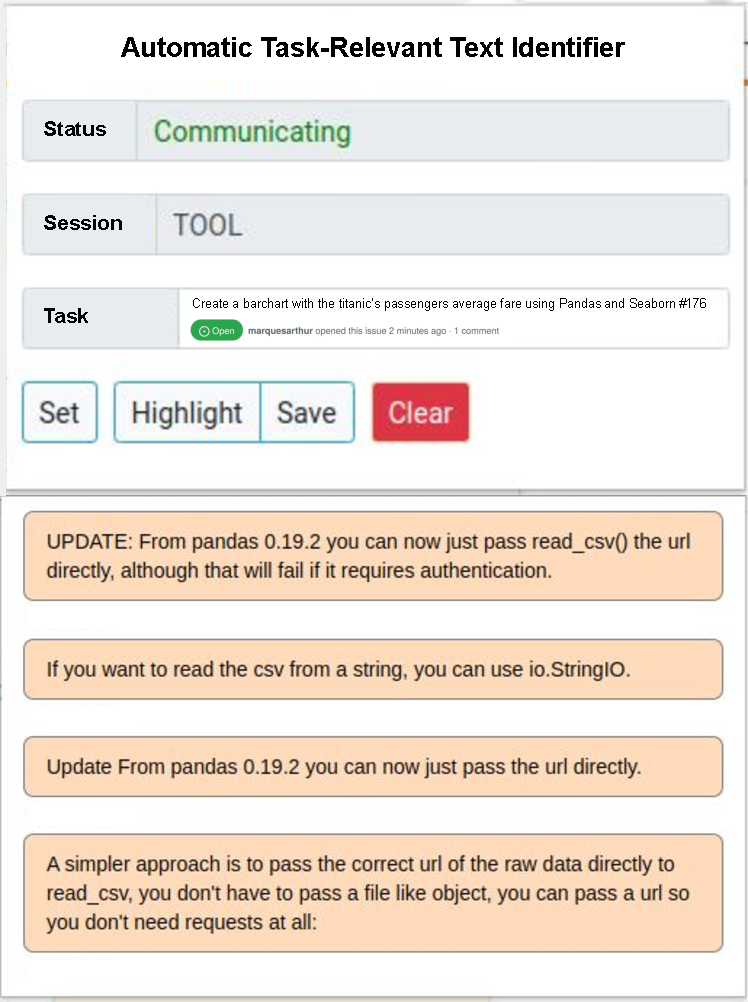
\includegraphics[width=0.5\textwidth]{fig/cp7/navigational-cues}
    \caption{Mock up of the highlights identified by \acs{tool} as navigational cues; by clicking on a highlight, a user could be directed to the part of a document containing that highlight}
    \label{fig:navigational-cues}
\end{figure}



A second approach to organizing the text identified could consider 
the semantic meaning of each sentence, as extracted through frame semantics or other semantic-based approaches. 
For instance, semantic frames could 
assist a user in comprehending the content of the text automatically identified
without the need to read it. 
Similar to Libra~\cite{Ponzanelli2017}, semantic frames could also be used to group the text identified in bubbles or a hierarchical representation 
 helping a developer
in deciding what portions of the text they would inspect first. 
Figure~\ref{fig:semantic-cues} shows a mock up 
with some of the semantic frames extracted 
for the sentences in Figure~\ref{fig:navigational-cues}.
Using the semantic frames identified,
a developer could decide whether they would read sentences 
describing some coding procedure (\textit{execution}), or sentences 
with warnings or requirements (\textit{requirement} and \textit{being obligated})
about the Pandas API. 
To be useful, future research must consider how to identify 
which frames, from all the frames available in a sentence, 
better summarize the meaning of the text. 







\begin{figure}[H]
    \centering
    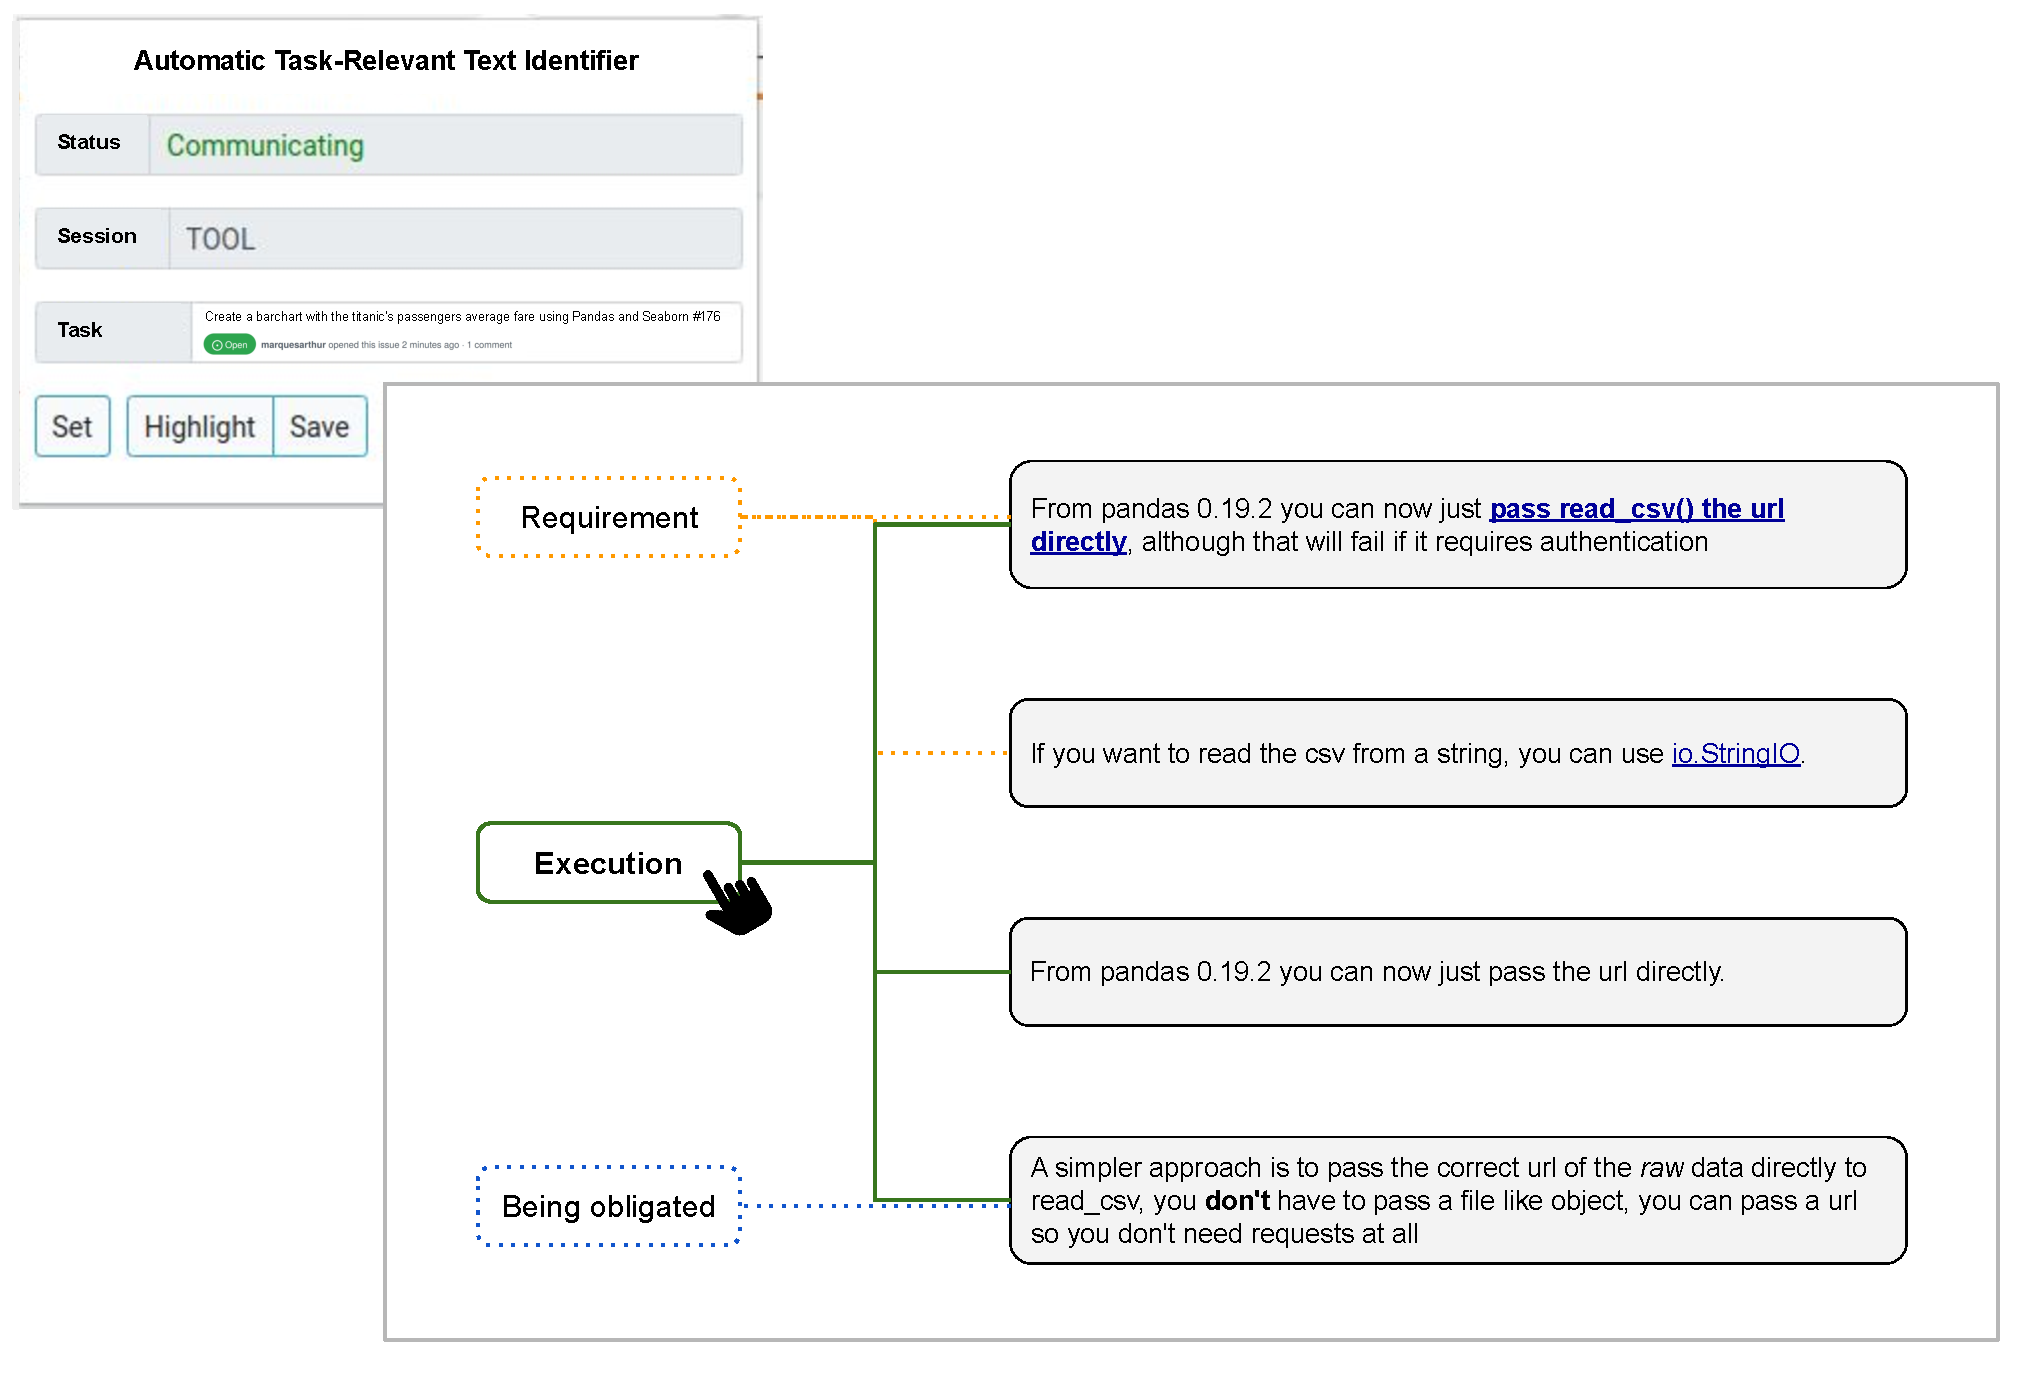
\includegraphics[width=0.95\textwidth]{fig/cp7/semantic-cues}
    \caption{Mock up of the highlights grouped by semantic frames; by hovering over a semantic frame, a user could quickly identify which of the text identified is associated with a certain semantic frame}
    \label{fig:semantic-cues}
\end{figure}






